\chapter{Segmentations}

\begin{figure}[ht!]
\centering
\begin{subfigure}[b]{0.7\textwidth}
   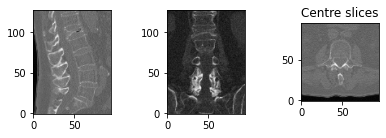
\includegraphics[width=1\linewidth]{images/results_2/original.png}
   \caption{Original image}
   \label{fig:Ng1} 
\end{subfigure}

\begin{subfigure}[b]{0.7\textwidth}
   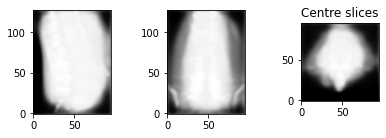
\includegraphics[width=1\linewidth]{images/results_2/binary_mask.png}
   \caption{Predictions of Model 1}
   \label{fig:Ng2}
\end{subfigure}

\begin{subfigure}[b]{0.7\textwidth}
   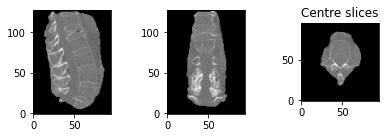
\includegraphics[width=1\linewidth]{images/results_2/binary_segmented.png}
   \caption{Segmented image with Model 1}
   \label{fig:Ng3}
\end{subfigure}

\begin{subfigure}[b]{0.7\textwidth}
   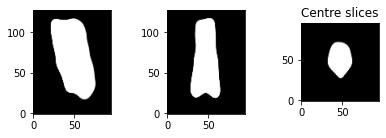
\includegraphics[width=1\linewidth]{images/results_2/dice_mask.png}
   \caption{Predictions of Model 2}
   \label{fig:Ng4}
\end{subfigure}

\begin{subfigure}[b]{0.7\textwidth}
   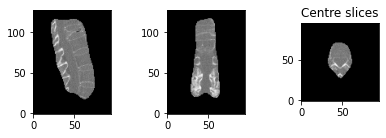
\includegraphics[width=1\linewidth]{images/results_2/dice_segmented.png}
   \caption{Segmented image with Model 2}
   \label{fig:Ng5}
\end{subfigure}

\caption[Results of spine segmentation]{Original and segmented CT image of a spine using Model 1 and Model 2.}
\label{fig:spine-segmentations-1}
\end{figure}

%--------------------------------------------------------------

\begin{figure}[ht!]
\centering
\begin{subfigure}[b]{0.7\textwidth}
   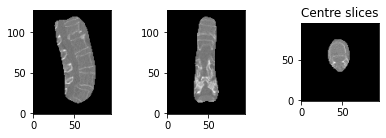
\includegraphics[width=1\linewidth]{images/results_4/1.png}
   \label{fig:Ng1} 
\end{subfigure}

\begin{subfigure}[b]{0.7\textwidth}
   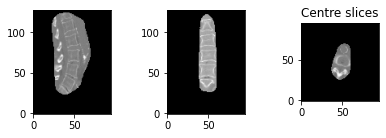
\includegraphics[width=1\linewidth]{images/results_4/2.png}
   \label{fig:Ng2}
\end{subfigure}

\begin{subfigure}[b]{0.7\textwidth}
   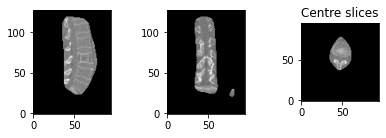
\includegraphics[width=1\linewidth]{images/results_4/3.png}
   \label{fig:Ng3}
\end{subfigure}

\begin{subfigure}[b]{0.7\textwidth}
   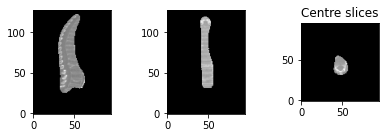
\includegraphics[width=1\linewidth]{images/results_4/4.png}
   \label{fig:Ng4}
\end{subfigure}


\caption[Results of spine segmentation with Model 2]{Segmented images with Model 2}
\label{fig:spine-segmentations-2}
\end{figure}